\documentclass[12pt]{article}
\usepackage{jmlda}
\usepackage{mathtext}
\usepackage{graphicx}
\usepackage{placeins}
%\NOREVIEWERNOTES
\title
    [Тематический поиск схожих дел в коллекции актов арбитражных судов] % Краткое название; не нужно, если полное название влезает в~колонтитул
    {Тематический поиск схожих дел в коллекции актов арбитражных судов}
\author
    [Герасименко~Н.\,А.] % список авторов для колонтитула; не нужен, если основной список влезает в колонтитул
    {Герасименко~Н.\,А., Артёмова~Е.\,Л., Воронцов~К.\,В.} % основной список авторов, выводимый в оглавление
    [Герасименко~Н.\,А.$^1$, Артёмова~Е.\,Л.$^2$, Воронцов~К.\,В.$^3$] % список авторов, выводимый в заголовок; не нужен, если он не отличается от основного
\thanks
    {Задачу поставил:  Воронцов~К.\,В.
    Консультант:  Артёмова~Е.\,Л.}
\email
    {nikgerasimenko@gmail.com}
\organization
    {$^1$МАИ; $^2$НИУ ВШЭ; $^3$МФТИ}
\abstract
    {В работе рассматривается задача информационного поиска по коллекции актов арбитражных судов. В качестве запроса поисковой системе может выступать любой документ коллекции. В ответ на поисковый запрос генерируется список документов коллекции, ранжированный по убыванию релевантности. Для решения поставленной задачи построена тематическая модель коллекции актов арбитражных судов с помощью открытой библиотеки BigARTM. При построении модели  учтена специфика предметной области: добавлены модальность ссылок на нормативно-правовые акты, а также модальность юридических терминов, выделенных полуавтоматически, с использованием алгоритма TopMine.


\bigskip
\textbf{Ключевые слова}: \emph {LegalTech, BigARTM, тематическое моделирование, аддитивная регуляризация мультимодальных иерархических тематических моделей}.}

\begin{document}
\maketitle
%\linenumbers
\section{Введение}

%Целью данной работы является построение тематической модели коллекции актов арбитражных судов для осуществления разведочного поиска по ней.

%Разведочный поиск - это относительно новая парадигма информационного поиска, отличающаяся тем, что позволяет подавать на вход поисковой системе не короткий запрос, а целый документ или коллекцию документов. 

%Разведочный поиск - это относительно новая парадигма информационного поиска, предполагающая 

Специалисты в области юриспруденции регулярно сталкиваются в своей работе с необходимостью поиска документов в базах судебной практики. Зачастую они ищут дела, схожие с теми, над которыми работают, не всегда при этом зная, по какому запросу или в какой именно тематике искать. Данная задача может быть отнесена к классу задач информационного поиска.

Существует несколько парадигм информационного поиска, одной из которых является тематический разведочный поиск, в рамках которого в качестве запроса может выступать целый документ или даже коллекция документов.

%Данная задача может быть рассмотрена как задача тематического разведочного поиска и решить ее с помощью разработанных методов решения этой задачи.

Юридические тексты обладают особой спецификой и, не смотря на то, что могут иногда казаться обычными текстами на естественном языке, не могут в полной мере рассматриваться таким образом. Понимание истинного смысла юридического текста зачастую требует консультации с экспертом.

В ходе совместной работы с экспертами в области юриспруденции был выявлен ряд важных модальностей, без учета которых невозможно построение адекватной модели. Библиотека BigARTM\cite{BigARTM2015}, с помощью которой строится тематическая модель, обладает возможностями для учета этих модальностей. В данной работе учтена модальность ссылок на нормативно-правовые акты и модальность юридических терминов.

%Представляется перспективным применение системы тематического поиска для решения подобной задачи. 


%Целью данной работы является построение тематической модели коллекции актов арбитражных судов для осуществления разведочного поиска. 

%Такого рода поиск называется разведочным\cite{Ianina_2017}.

%, для его осуществления разработано множество методов. В данной работе сделана попытка применения одного из методов разведочного поиска, основанного на построении тематической модели, к задаче поиска по коллекции юридических документов.

%Для построения тематической модели используется библиотека BigARTM\cite{BigARTM2015}. Одним из ее преимуществ является возможность учета модальностей, с помощью которого сделана попытка учесть специфику предметной области, выделив ссылки на нормативно-правовые акты и юридические термины. Задача выделения именованных сущностей решается с помощью регулярных выражений и алгоритма TopMine для выделения коллокаций.

%модальности позволяют учесть дополнительную информацию при построении модели
%это очень важно, потому что область обладает большой специфичностью

Данное исследование основано на подходе, описанном в работе \cite{Ianina_2017}, где он использован при построении тематической модели для разведочного поиска по статьям на порталах Habrahabr.ru и TechCrunch.com. Построенная авторами модель показала хорошие результаты на размеченных с помощью ассесоров данных.

\section{Постановка задачи}

Дана коллекция, состоящая из 7937 юридических документов, а именно актов арбитражных судов относящихся к делам о банкротстве. Для каждого документа известно его место в иерархии категорий, например, категория <<Особенности банкротства отдельных категорий должников>> или подкатегория <<Внешнее урправление>>  категории <<Процедры банкротства>>.

Задача состоит в построении тематической модели данной коллекции с помощью библиотеки BigARTM. Перед построением тематической модели необходимо провести предварительную обработку текстов, которая заключается в следующих шагах.
\begin{enumerate} 
  \item Проанализировав структуру документов, требуется выделить из них, при помощи контекстно-свободных грамматик и регулярных выражений, ссылки на нормативно-правовые акты (НПА).
  \item Требуется выделить юридические темины с помощью алгоритма TopMine \cite{El-Kishky2014}.
\end{enumerate}
Ссылки на НПА и юридические термины будут учтены в модели в качестве модальностей.

%Предварительная оценка модели будет проводиться по критериям перплексии и разреженности, а окончательная - по методу, описанному в работе \cite{Ianina_2017}, а также на странице русскоязычного вики-ресурса MachineLearning.ru «Оценивание качества разведочного поиска (эксперимент)», основанная на асессорских оценках релевантности.

Предварительная оценка модели будет проводиться по критериям перплексии, разреженности распределений тем в документах, а также разреженности распределений токенов в темах для модальностей ссылок на НПА и юридических терминов в соответствии со стандартной методологией оценки \cite{vorontsov2015additive}. 

Окончательная оценка будет строиться следующим образом. Полученные в результате моделирования тематические вектора для каждого документа кластеризуются при помощи алгоритма k-means. Затем, по критерию Rand Index делается оценка, в какой степени картина кластеризации согласованна с картиной принадлежности документов их категориям:  оказались ли в одном кластере документы из одной категории, и оказались ли документы из разных категорий в разных кластерах.

Таким образом, формальная постановка задачи может быть сформулирована в следующем виде.
Пусть $D$ - коллекция документов, $|D|=n$. Каждый документ $d\in D$ принадлежит одной из категорий $T_{i}\in T$. С другой стороны, каждый документ $d$ принадлежит одному из кластеров $Y_{j}\in Y$, полученных в результате применения алгоритма k-means к множеству тематических векторов документов коллекции. Требуется построить тематическую модель таким образом, что


\begin{align*}
\frac{a+b}{a+b+c+d} = \frac{a+b}{{n \choose 2 }}\to max,
\end{align*}

где:

$a = |S^{a}|,$ где $S^{a} = \{ (d_{i}, d_{j}) \mid d_{i}, d_{j} \in Y_{k}, d_{i}, d_{j} \in T_{l}\},$

$b = |S^{b}|,$ где $S^{b} = \{ (d_{i}, d_{j}) \mid d_{i} \in Y_{k_{1}}, d_{j} \in Y_{k_{2}}, d_{i} \in T_{l_{1}}, d_{j} \in T_{l_{2}}\},$

$c = |S^{c}|,$ где $S^{c} = \{ (d_{i}, d_{j}) \mid d_{i}, d_{j} \in Y_{k}, d_{i} \in T_{l_{1}}, d_{j} \in T_{l_{2}}\},$

$d = |S^{d}|,$ где $S^{d} = \{ (d_{i}, d_{j}) \mid d_{i} \in Y_{k_{1}}, d_{j} \in Y_{k_{2}}, d_{i}, d_{j} \in T_{l}\},$

$1 \leq i,j \leq n, i \neq j, 1 \leq k, k_{1}, k_{2} \leq r, k_{1} \neq k_{2}, 1 \leq l, l_{1},l_{2} \leq s, l_{1} \neq l_{2}.$


\section{Вероятностное тематическое моделирование на основе аддитивной регуляризации}

Пусть $M$ - множество модальностей, каждой из которой соответствует набор токенов $W_{m}$, называемый словарем модальности. Пусть $W$ - множество токенов из всех словарей, соответствующих модальностям из $M$. Каждый документ коллекции $D$ с длинной ${n_{d}}$  представляет собой набор токенов $w_{1},...,w_{n_{d}}$ из множества $W$.

В соответствии с теорией аддитивной регуляризации тематических моделей для каждой модальности вводится критерий логарифма правдоподобия и с помощью EM-алгоритма максимизируется их взвешенная сумма. Также к сумме добавляются регуляризаторы - дополнительные критерии, необходимые поскольку в общем случае задача имеет бесконечно много решений.

\emph{Регуляризаторы сглаживания и разреживания} имеют одинаковый вид и отличаются только знаками коэффициентов $\alpha$ и $\beta$, для регуляризатора разреживания они отрицательны.
\begin{equation}
R(\Phi,\Theta)=\beta \sum_{m \in M}\sum_{t \in T}\sum_{w \in W^m} \beta_{w} ln \phi_{wt} + \alpha \sum_{d \in D}\sum_{t \in T}\alpha_{t} ln\theta_{td}\to max.
\end{equation} 
Регулятор сглаживания вводит в модель требование схожести распределений $\phi_{wt}$ с распределением $\beta_{w}$ и $\theta_{td}$ с распределением $\alpha_{t}$. Регуляризатор разреживания, в свою очередь, способствует появлению нулевых элементов в распределенях $\phi_{wt}$ и $\theta_{td}$, что позволяет находить более компактные представления документов.

\emph{Регуляризатор декоррелирования} вводит в модель требование различности тем путем минимизации ковариации между столбцами матрицы $\Phi$.
\begin{equation}
R(\Phi)=-\tau \sum_{t \in T}\sum_{s \in T\backslash t}\sum_{w \in W} \phi_{wt}\phi_{ws} \to max.
\end{equation} 
Также побочным эффектом работы регуляризатора декоррелирования является разреживание матрицы $\Phi$, поэтому в случае его применения, можно не применять регуляризатор разреживания для нее.

\section{Вычислительный эксперимент}
Эксперимент проводился на коллекции, состоящей из 7937 юридических документов, а именно актов арбитражных судов относящихся к делам о банкротстве. О каждом документе была известна его категория, 
эта информация в последствии использовалась для внешней оценки качества модели. При построении модели использовались, помимо модальности текста, модальность ссылок на НПА и модальность юридических терминов. 

В рамках предобработки документов была проведена лемматизация при помощи морфологического анализатора pymorphy2, были исключены 5\% наиболее высокочастотных слов, а также слова общей лексики из списка stop-words библиотеки nltk.

При построении тематической модели использовались регуляризаторы декоррелирования для матрицы $\Phi$ терминов в темах и регуляризатор разреживания для матрицы $\Theta$ тем в документах. Выбор параметров модели производился путем перебора значений по сетке с использованием набора критериев качества: перплексия, разреженность распределений токенов в темах, разреженность распределений тем в документах, в также внешнего критерия качества. Подбор весов модальностей также производился с помощью перебора по сетке.

Для каждого значения параметра регуляризации производилось по 8 итераций EM-алгоритма, после чего выбиралось то значение, при котором модель улучшилась по одному или нескольким критериям качества, существенно не ухудшившись ни по одному из них. 

Регуляризатор декоррелирования матрицы $\Phi$ добавлялся в модель изначально, а спустя 8 итераций EM-алгоритма добавлялся регуляризатор разреживания для матрицы $\Theta$. 

На рисунке 1 изображены графики зависимости перплексии и разреженности распределений терминов в темах модели при найденных оптимальных значениях параметров регуляризации: $\tau = 3100$, $\alpha = -1.5$, $\beta = 0.25$.

В ходе сравнения показателей внешнего критерия качества - согласованности кластеризации тематических векторов и принадлежности документов категориям - модели АРТМ и модели tf-idf ссылок на НПА получены результаты, отраженные в таблице \ref{tab:summary}.


\begin{figure}[H]
  \subfloat[Перплексия (термины)]{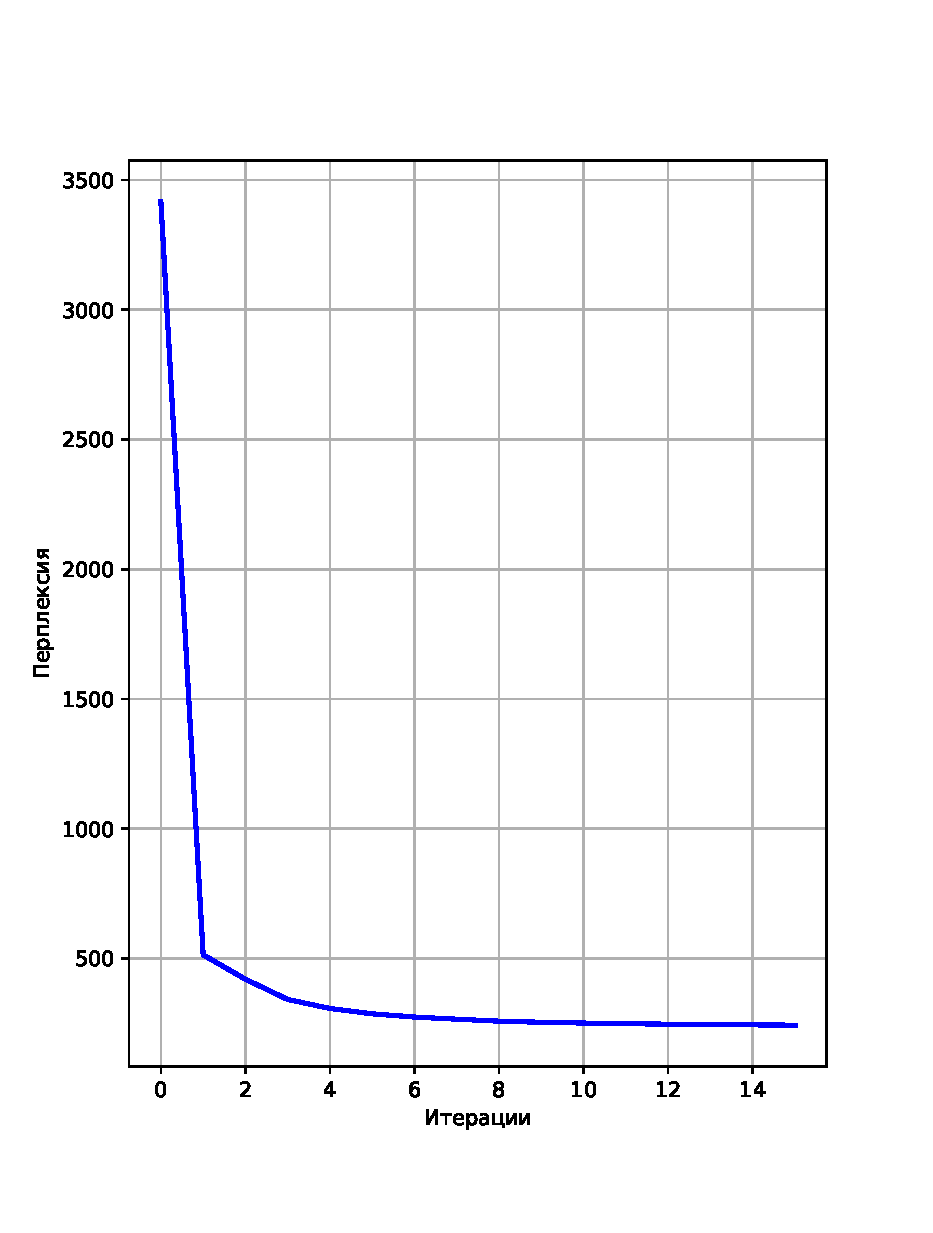
\includegraphics[width=0.5\textwidth]{perplexity}}
  \subfloat[Разреженность $\Theta$ (термины)]{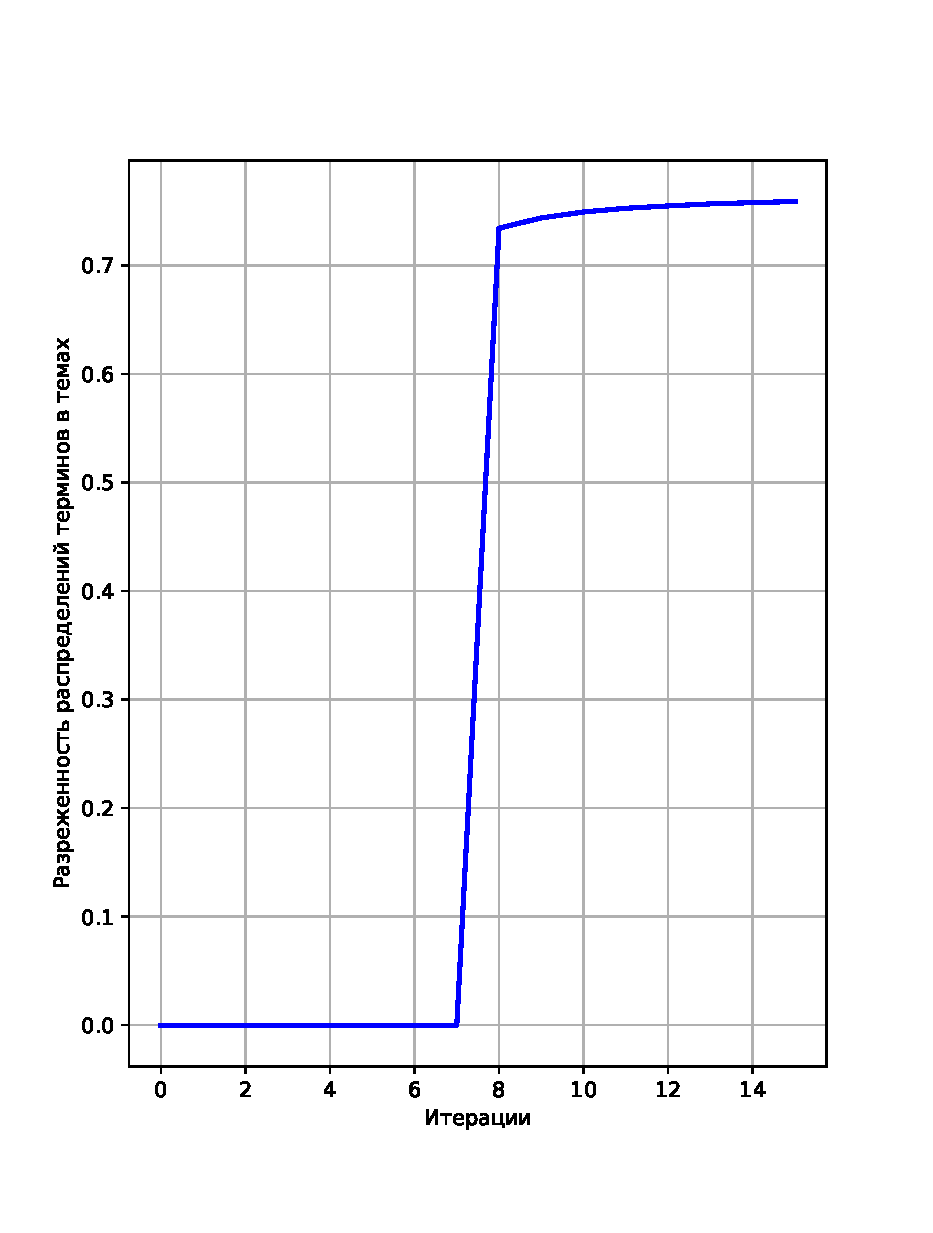
\includegraphics[width=0.5\textwidth]{sparseTheta}}\\
\caption{Зависимости перплексии и разреженности распределений терминов в темах.}
\label{fg:Example}
\end{figure}

\begin{table}[H]
\caption{\label{tab:summary}Сравнение показателей внешнего критерия качества.}
\begin{center}
\begin{tabular}{|c|c|c|}
\hline
Модель & ARI & AMI\\
\hline
TF-IDF по словам & 2\% & 2.5\% \\
\hline
TF-IDF по ссылкам на НПА & 17\% & 22\% \\
\hline
АРТМ & 37.5\% & 42\% \\
\hline
\end{tabular}
\end{center}
\end{table}


\section{Заключение}
Целью разведочного поиска является облегчение для человека задачи поиска необходимой информации, и поиск для специальстов в области юриспруденции является конкретной реализацией этой идеи. В работе рассмотрена задача информационного поиска по коллекции юридических документов, а именно актов арбитражных судов. 

При помощи библиотеки BigARTM построена тематическая модель, строющая для документов коллекции сжатые векторные представления и, таким образом, позволяющая реализовать поиск, используя косинусную меру близости.

Был реализован метод внешней оценки качества тематической модели, заключающийся в вычислении согласованности между картиной кластеризации тематических векторов документов коллекции и их принадлежности различным категориям дел.

Результаты показывают, что тематическая модель способна корректно строить векторные представления юридических документов, что, в перспективе, дает возможность построения системы разведочного поиска, с использованием тематического моделирования в качестве ключевой технологии.



%Регуляризаторы добавлялись в тематическую модель по очереди: сначала 8 итераций EM-алгоритма с регуляризатором декоррелирования матрицы $\Phi$, затем добавляется регуляризатор разреживания матрицы $\Theta$ еще на 8 итераций.  

%Процедура подбора параметров регуляризации состояла в следующей последовательности действий для каждого параметра :
%\begin{enumerate}
%\item Добавление регуляризатора декоррелирования для матрицы $\Phi$ терминов в темах
%\item Произведение 8 итераций EM-алгоритма
%\item Оценка модели по внутренним и внешним критериям качества 
%\item Добавление регуляризатора разреживания для матрицы $\Theta$ тем в документах
%\item Произведение 8 итераций EM-алгоритма
%\item Оценка модели по внутренним и внешним критериям качества
%\end{enumerate}





\bibliographystyle{plain}
\bibliography{Gerasimenko2019Project50}


\end{document}
